\begin{refsegment}
\chapter{GROOLS}

Ces trois années de recherche ont été consacrées à la conception d’une méthode et au développement du logiciel \gls{GROOLS} . Ce logiciel offre une approche interactive entre le biologiste et les prédictions bio-informatiques lors du processus de curation de l'annotation fonctionnelle des génomes bactériens au travers de processus biologiques comme les voies métaboliques. Compte tenu de l'augmentation constante et rapide des annotations automatiques, un système expert pourrait aider les biologistes à détecter les annotations inconsistantes et contradictoires dans cette masse d'information. 

\section{Le début de GROOLS}

\subsection{HERBS}

L'équipe \texttt{HELIX} d'\textit{Alain VIARI} avait commencé un projet en ce sens nommé \texttt{\gls{HERBS}} en collaboration avec le \texttt{\gls{SIB}} dans le cadre du projet \gls{HAMAP} \cite{pedruzzi2015hamap}. L'objectif de \texttt{\gls{HERBS}} est d'alerter les biologistes sur les fonctions et les voies métaboliques manquantes, non attendues ou encore ambiguës. Pour cela l'outil s'appuie sur le moteur d'inférence \texttt{\gls{JESS}}, sur une base de connaissances (contenant les règles et les faits, \cref{fig:systeme_expert}) et sur une interface graphique pour l'exploration des connaissances. 

Les connaissances dans \texttt{HERBS} sont structurées en trois composants :\nolisttopbreak
\begin{itemize}
	\item Une Base de Connaissance qui contient des faits primaires sur l’organisme étudié (sa taxonomie  et des propriétés phénotypiques, exemple : l’organisme est photosynthétique) et des faits généraux décrivant des processus biologiques et leurs composants sous la forme d’un  graphe orienté acyclique avec des nœuds \texttt{ET} et \texttt{OU}.
	\item Une Base d’Observations qui contient des prédictions d’unités fonctionnelles (i.e. composants de processus) dans l’organisme étudié.
	\item Des règles logiques permettant de prendre des décisions (e.g. SI X est requis par une bactérie et X n’est pas observé ALORS X est manquant dans l’annotation de la bactérie).
\end{itemize}

Le raisonnement dans \texttt{HERBS} se fait en propageant les observations au travers du graphe de connaissances par l’application des règles logiques. Chaque nœud est associé à trois attributs pouvant prendre les valeurs oui ou non au cours du raisonnement :\nolisttopbreak
\begin{itemize}
	\item "Présent", le composant est prédit ou non dans l’organisme
	\item "Requis", le composant est attendu dans l’organisme (i.e. il doit être prédit)
	\item "Interdit", le composant n’est pas attendu dans l’organisme.
\end{itemize}

À la fin du raisonnement des conclusions sur les processus et leurs composants sont données suivant cette table de correspondance :\nolisttopbreak
\begin{table}[H]
	\centering
	\begin{tabular}{|l|l|l|>{\columncolor{LightCyan}}l|}
		\toprule
		\rowcolor{LightCyan}
		\textbf{Présent} & \textbf{Requis} & \textbf{Interdit} & \textbf{Conclusion} \\ 
		\midrule
		oui & oui & oui & ambigu \\ 
		\hline 
		oui & oui & non & normal \\ 
		\hline 
		oui & non & oui & inattendu \\ 
		\hline 
		oui & non & non & orphelin \\ 
		\hline 
		non & oui & oui & ambigu \\ 
		\hline 
		non & oui & oui & manquant \\ 
		\hline 
		non & non & oui & normal \\ 
		\hline 
		non & non & non & normal \\ 
		\bottomrule
	\end{tabular} 
\end{table}

\textit{Alain VIARI} m'a permis d'utiliser l'outil \texttt{PathRules} qui est une implémentation de \texttt{\gls{HERBS}} avec le moteur \texttt{\gls{CLIPS}} \cite{riley1991clips}.


Pour tester le logiciel \texttt{PathRules} j'ai fourni à la base de faits les voies de biosynthèse de la lysine avec le variant (\texttt{AAA} et le variant \texttt{DAP}) décrits par \texttt{UniPathway} et les prédictions d’activités enzymatiques provenant de l’analyse 79 génomes. Pour ce faire les données sont rangées dans trois dossiers présents à la racine du projet: (i) \texttt{data/processes} pour la description des voies métaboliques, (ii) \texttt{data/observers/uniprot} pour le catalogues des prédictions par espèces, (iii) \texttt{data/species} pour la description taxonomique des espèces. Les fichiers doivent porter l'extension \texttt{.data} et le nom du fichier est utilisé comme identifiant pour faire le lien entre les processus, les prédictions et les informations taxonomiques de l'espèce. Par exemple, j'ai utilisé l'identifiant \texttt{ACIAD} pour mettre en relation les informations d'\textit{Acinetobacter baylyi ADP1}.

\console{find data/ -name 'ACIAD.data'}{ data/observers/uniprot/ACIAD.data\par data/species/ACIAD.data }


La description des données dans ces fichiers suit la nomenclature \texttt{\gls{CLIPS}}. C'est-à-dire que les faits sont déclarés entre parenthèses. C'est la raison pour laquelle les observations sont formatées comme suit: 

( \texttt{source} (id \texttt{xxx}) (alias \texttt{yyy} sp:\texttt{zzz})  )

Extrait d'un fichier cataloguant les faits relatifs à une espèce:\nolisttopbreak

\console{head data/observers/uniprot/data/ACIAD.data}{
    (uniprot (id ASPARTATE-SEMIALDEHYDE-DEHYDROGENASE-RXN) (alias ACIAD0479 sp:ACIAD00423))\par
    (uniprot (id SUCCDIAMINOPIMDESUCC-RXN) (alias ACIAD0791 sp:ACIAD0070)\par
    (uniprot (id ASPARTATEKIN-RXN) (alias ACIAD1252 sp:ACIAD01133))\par
    (uniprot (id SUCCINYLDIAMINOPIMTRANS-RXN) (alias ACIAD2080 sp:ACIAD01886))\par
    (uniprot (id TETHYDPICSUCC-RXN) (alias ACIAD2599 sp:ACIAD02357))\par
    (uniprot (id DIAMINOPIMEPIM-RXN) (alias ACIAD2659 sp:ACIAD02412))\par
    (uniprot (id DIAMINOPIMDECARB-RXN) (alias ACIAD2660 sp:ACIAD02413))\par
    (uniprot (id DIHYDRODIPICSYN-RXN) (alias ACIAD3585 sp:ACIAD03222))\par
    (uniprot (id DIHYDROPICRED-RXN) (alias ACIAD3619 sp:ACIAD03252))\par
}


L'information taxonomique est également un fait. Il débute par "species" suivis de plusieurs chaînes de caractères pour renseigner de plus en plus précisément la taxonomie de l'organisme.

\console{cat data/species/ACIAD.data}{ (species lineage Bacteria Proteobacteria Gammaproteobacteria Pseudomonadales Moraxellaceae Acinetobacter Acinetobacter\_sp.\_ADP1) }

Pour représenter la structure hiérarchique des voies métaboliques, les faits sont organisés pour exprimer la notion de composition et d'équivalence. La notion de composition et utilisé pour relier les ensembles de réactions (\gls{ULS} \texttt{d’UniPathway}) à leurs réactions. Quant à l'équivalence elle permet de définir les chemins alternatifs (variants) pour réaliser une voie métabolique. La syntaxe \texttt{\gls{CLIPS}} utilise $x -> \ldots$ pour signifier "x tel que \ldots". La partie à droite de la flèche décrit les relations en notation polonaise\footnote{Également connue sous le nom "notation pré-fixée". Par exemple, le calcul "$5 \times (2 + 3)$", s'écrit "$\times 5 (+ 2 \qquad 3)$". }. Ci-après le fichier de description de la voie métabolique de la biosynthèse de la lysine par le variant \texttt{AAA} (Acide alpha-Amino Adipique) selon \texttt{UniPathway}.

\console{cat data/processes/lysine\_AAA\_biosynthesis.data}{
;;;; --------------------------------------------------------\par
;;; HERBS (Hamap Expert Rules Based System)\par
;;;\par
;;; @file: lysine\_AAA\_biosynthesis.data\par
;;; --------------------------------------------------------\par
;;;\par
(process declare lysine\_AAA\_biosynthesis present in ALL)\par
(process define lysine\_AAA\_biosynthesis -> and UPA00033)\par
(process define UPA00033 -> or UPA00033-alt-0 UPA00033-alt-1)\par
(process define UPA00033-alt-0 -> and ULS00012 ULS00013)\par
(process define UPA00033-alt-1 -> and ULS00012 ULS00014)\par
(process define ULS00012 -> and ULS00012-alt-0)\par
(process define ULS00012-alt-0 -> and UER00028 UER00029 UER00030 UER00031 UER01027)\par
(process define ULS00013 -> or ULS00013-alt-0 ULS00013-alt-1)\par
(process define ULS00013-alt-0 -> and UER00032 UER00034)\par
(process define ULS00013-alt-1 -> and UER00033 UER00034)\par
(process define ULS00012 -> and ULS00012-alt-0)\par
(process define ULS00012-alt-0 -> and UER00028 UER00029 UER00030 UER00031 UER01027)\par
(process define ULS00014 -> or ULS00014-alt-0 ULS00014-alt-1)\par
(process define ULS00014-alt-0 -> and UER00035 UER00037 UER00038 UER00039)\par
(process define ULS00014-alt-1 -> and UER00036 UER00037 UER00038 UER00039)\par
}


Chaque processus est un fait, désigné par le mot clé "process". Les voies métaboliques sont préfixées du mot clé "declare" et "define" pour ses composants. Les faits constituant la voie métabolique sont hiérarchiquement organisé. Lorsqu'un fait est composé de plusieurs concepts on utilise le symbole "and" et le symbole "or" lorsqu'un fait possède des équivalences. Les lignes débutant par un point virgule ne sont pas interprétées par  \texttt{\gls{CLIPS}}.Elles permettent de commenter les règles et les faits.

À la fin du raisonnement, une évaluation de la complétion de l'annotation fonctionnelle des génomes est proposée sous la forme d’un tableau(\cref{fig:herbs_rapport}).

\begin{shadedfigure}[H]
    \centering
    \includegraphics[width=\textwidth]{img/herbs_conclusion_report.png}
    \caption{Rapport sur la présence de la voie de biosynthèse de la lysine.}
    \label{fig:herbs_rapport}
\end{shadedfigure}

L'utilisateur a la possibilité d'explorer les résultats de \texttt{\gls{HERBS}} sur les voies métaboliques et leurs composants à travers un graphe orienté acyclique (\cref{fig:herbs_dag}).

\begin{landscape}
    \begin{shadedfigure}[H]
        \centering
        \includegraphics[width=\textwidth]{img/herbs_aciad_lysine_dap.png}
        \caption{Rapport sur la présence de la voie de biosynthèse de la lysine. La couleur jaune indique que la prédiction portée sur le concept est en accords avec les connaissances acquises sur l'organisme. Dans le cas contraire le concept est sur fond rouge. }
        \label{fig:herbs_dag}
    \end{shadedfigure}
\end{landscape}


Pour passer à l'échelle, il est nécessaire de retranscrire  en \texttt{\gls{CLIPS}}  toutes les voies métaboliques et toutes les prédictions bio-informatiques. De plus le système doit être étendu à la notion d'inconnu et si possible à la notion de contradiction. Car en biologie, l’absence de résultat suite à une expérience ou à une prédiction est souvent difficile à interpréter comme un résultat vrai négatif ou faux négatif.  Dans le but d'appuyer le propos sur l'intérêt de valeurs autres que frai et faux, une non-prédiction bio-informatique ne signifie pas une prédiction de non-présence. Ce point de vue peut paraître un peu philosophique. Il fait référence aux concepts de "monde ouvert" et "monde fermé". Une hypothèse en monde fermé va considérer toutes les questions sans réponse comme fausses. En monde ouvert, les hypothèses prennent les valeurs vraies ou fausses lorsqu'elles sont explicitement décrites comme telles. Pour les autres cas, une hypothèse est considérée incertaine tant qu'un fait ne la désigne pas comme vraie ou fausse. En biologie quantité de connaissances ne sont pas prédites et pour autant cela ne signifie pas qu'elles sont prédites comme non présentes dans l'organisme. Dans l’exemple précédent de \texttt{\gls{HERBS}}, la plupart des voies métaboliques sont déclarées "Missing" sans pour autant suggérer quel variant est le plus probable pour l'organisme d'intérêt. Ceci est s'explique d'une part à cause des prédictions bio-informatiques, elles sont soit présentes soit non présentes (équivalant à ni-vrai-ni-faux) par conséquent il n'y a pas de prédiction pour indiquer l'absence d'une fonction. D'autre part le système n'est pas capable de choisir lorsque les prédictions ne couvrent pas l'ensemble d'un variant ce qui est justement la problématique en biologie. La combinaison de ces deux cas induit que la plupart des voies métaboliques seront soit "Missing" lorsque la voie est requise soit "Normal" si elle est ni requise ni interdites. On pourrait s’attendre à ce que le système \texttt{\gls{HERBS}} soit capable de repérer les variants requis pour corréler les attentes portées sur les voie métaboliques.

\subsection{Contexte du projet GROOLS}

Mon projet de recherche a débuté par l'identification des besoins et des outils à ma disposition. Les besoins de la plateforme \texttt{MicroScope} (i.e. plateforme d’annotation de génomes microbiens, développée dans le laboratoire où j’ai réalisé ces travaux) se divisent en trois axes.

Le premier  correspond à la modernisation du système de gestion et déclaration des chaînages applicatifs ("wokflows"). Pour cela la plateforme \texttt{MicroScope} s'oriente vers la mise en place du moteur à base de règles développé en interne au \texttt{GenoScope} (\texttt{\gls{BIRDS}}) . Le système utilise l'application \texttt{DROOLS}\cite{mcwhirter2001drools,browne2009jboss} pour raisonner et donc ordonnées les processus à partir de règles métiers décrivant les ressources à utiliser et l’enchainement des programmes dans le processus de l'annotation.

Le second axe consiste à la mise en place d'un système d'intégration des données métabolique de la plateforme, dénommé \texttt{Galileo} \cite{galileo2014}. Cet outil a la faculté de réconcilier les informations provenant de multiple ressources externes et internes et donc d'avoir accès à un large éventail d'information à travers une unique interface. Ceci permet  notamment de fournir une représentation unifiée des connaissances métaboliques par l'utilisation des informations de \texttt{ChEBI} \cite{hastings2013chebi}, \texttt{RHEA} \cite{alcantara2012rhea}, \texttt{KEGG} et \texttt{MetaCyc}.

Le troisième axe s'articule autour d'un système à base de règles pour l'annotation des génomes. Il a pour objectif de guider le biologiste sur les annotations suspectées manquantes dans un organisme donné. Il est composé de deux modules. Le premier a pour objectif de récupérer les règles d'\texttt{UniRule} et de les rendre utilisable en dehors de "l'\gls{EBI}". Les règles d'annotation fonctionnelle à partir des domaines protéiques seraient ainsi partagées à la communauté scientifique. Le deuxième module doit évaluer les fonctions prédites au regard des processus métaboliques et mettre en évidence des annotations confirmées,   manquantes ou contradictoires. La cohérence des annotations d'un génome peut ainsi être évaluée au regard des attentes portées sur des processus que l'organisme est capable de réaliser. L'application \texttt{DROOLS} a été choisie pour la mise en œuvre du raisonnement afin de garder la maîtrise autour d'une même application pour tout développement impliquant un système à base de règles. Son moteur de règle se montre moderne et capable de communiquer avec les applications \texttt{Java} ce  qui est un avantage car \texttt{Galileo} et \texttt{BIRDS} sont également écrit dans ce même langage.

C'est sur ce dernier axe que j'ai effectué mes recherches tout en échangeant avec les deux premiers axes afin de récupérer les prédictions bio-informatiques et les données métaboliques unifiées. Le cadre de mon projet de recherche a été présenté lors de la 10$^{eme}$ conférence internationale sur l'intégration de données en science de la vie (DILS 2014 \url{http://dils2014.inesc-id.pt/}).

\includepdf[pages=-]{img/DILS_2014.pdf}

\subsection{Logique et notion d'objet}

Au début de mes investigations, j'ai rencontré plusieurs difficultés. La première était d'utiliser les données structurées et complexes issues de la biologie à travers des règles de logique. Il faut savoir que la plupart des raisonneurs (comme \texttt{Prolog} et \texttt{CLIPS}) utilise la programmation déclarative, ce qui consiste à décrire le problème\footnote{Par opposition a des langages comme Java, Python, D, Perl \ldots, ils utilisent la programmation impérative qui s'attache à décrire comment trouver la solution.}. La déclaration de problèmes impliquant  des données structurées n'était pas initialement prévue dans ce paradigme\footnote{Des extensions du paradigmes ont permis d'utiliser des structures de données complexes comme Prolog++.}. Par exemple un bloc de réactions composé des réactions A et B peut s'exprimer par la règle suivante (en Prolog):

\begin{lstlisting}[basicstyle=\small\normalfont\ttfamily,language=Prolog]
    reaction_block(Arg1, Arg2) :-
        reaction_A(Arg1),
        reaction_B(Arg2).
\end{lstlisting}

Ce qui précède  ":-" est le nom de la règle et ses arguments, ce symbole signifie "si". Pour reprendre l'exemple précédant "reaction\_block(Arg1,Arg2)" est vrai si "reaction\_A(Arg1)" et "reaction\_B(Arg2)" sont vrais. Il n'est pas simple de rattacher des attributs à des catégories de réaction comme on pourrait le faire avec le paradigme orienté-objet. C'est la raison pour laquelle j'ai utilisé le système \texttt{DROOLS}. Il permet d'utiliser des objets (au sens du langage Java)  et de les utiliser pour établir des règles. Par exemple, l'utilisation d'un attribut peut être employé pour indiquer que certaines réactions sont optionnelles et ainsi "relacher" la définition du bloc de réaction. Le raisonnement peut ainsi être orienté par les états des différents attributs attachés à une réaction. La représentation des connaissances sous forme d'objet permet également d'exprimer la composition d'autres objets, par exemple la déclaration d'une classe bloc de réaction avec pour attribut une liste d'objet de type réaction. Je devais donc établir un raisonnement logique utilisant des structures de données et leurs relations. Pour cela je me suis inspiré de la logique orientée-objet du premier ordre ("\citetitle{amir1999object}") \cite{amir1999object}, du projet \texttt{\gls{HERBS}} et utilisé l'application \texttt{DROOLS} pour écrire les règles de raisonnement et établir une description formelle des objets manipulés.

\subsection{Représentation des connaissances}

La seconde problématique portait sur la représentation des connaissances. Les voies métaboliques sont représentées de différentes manières selon la ressource utilisée. Il était nécessaire d'avoir un modèle hiérarchique des connaissances unifié pour avoir le même raisonnement indifféremment de la ressource métabolique utilisée. Pour cela, j'ai étudié les représentations des voies métaboliques de \texttt{Metacyc} (\cref{fig:metacyc_lysine}), \texttt{KEGG} (\cref{fig:kegg_lysine}) et \texttt{UniPathway} (\cref{fig:lysine}) et recherché les caractéristiques pouvant être mise en commun. Cette étude a permis de mettre en place une structuration hiérarchique de connaissances \textit{a priori} dans un graphe ET/OU. Je parle ici de connaissances \textit{a priori} car tant que les prédictions et les expectations n'ont pas été évalué la connaissance n'est pas validé. C'est la raison pour laquelle j'emploie également les termes de théorie et de concept en lieu et place de connaissance \textit{a priori}. 

Les observations sont reliées a ces connaissances \textit{a priori} pour indiquer les expectations et les prédictions sur les voies métaboliques. Les observations et les concepts sont des faits à partir desquels les règles logiques vont établir un raisonnement. 

\needspace{15\baselineskip}
\begin{lstlisting}[caption=Inférence de la prédiction d'absence, style=drl-style]
rule "Prediction infer his none existence" @\tikz[remember picture] \node [] (a){};@
when   @\tikz[remember picture] \node [] (b){};@
	$k: PriorKnowledge( $kid := id, nodeType == NodeType.LEAF )   @\tikz[remember picture] \node [] (c){};@
	( @\tikz[remember picture] \node [] (d){};@
		or
		not( Prediction( $kid := knowledgeId ) )
		Prediction( $kid := knowledgeId, presence == FourState.UNKNOWN )
	)
then @\tikz[remember picture] \node [] (e){};@
	modify( $k ){ 
		presence = FourState.UNKNOWN
	}
end
\end{lstlisting}
\begin{tikzpicture}[remember picture, overlay, every edge/.append style = { ->, thick, >=stealth, DimGray, dashed, line width = 1pt },
					every node/.append style = { align = center, minimum height = 10pt, font = \tiny, fill= green!20},
					text width = 2.5cm ]
	\node [above left = .8cm and 4.5 cm of a,text width = 2.2cm]
	(A) {Nom de la règle};
	\draw (A.south) + (0, 0) coordinate(x1) edge (x1|-a.north);	
	\node [right = 5.5cm of b, text width = 4cm]  (B) {Déclaration des contraintes};
	\draw (B.west) edge (b.east) ;
	\node [right = 1.5cm of c, text width = 3cm]  (C) {Sélection d'une Connaissance \textit{a priori} étant une feuille dans le graphe};
	\draw (C.west) edge (c.east) ;
	\node [below right = -0.2cm and 2cm of d, text width = 8cm]  (D) {Déclaration de deux propositions relié par l'opérateur OU};
	\draw (D.west) edge (d.east) ;
	\node [right = 4.cm of e, text width = 6cm]  (E) {Description de la conséquence logique lorsque la règle est vrai};
	\draw (E.west) edge (e.east) ;
\end{tikzpicture} 

Les connaissances \textit{a priori} sont reliées les unes aux autres par des relations pour exprimer la composition et l'équivalence. Pour cela l'attribut \texttt{NodeType} peut prendre la valeur AND/OR .

\needspace{15\baselineskip}
\begin{lstlisting}[caption=Inférence de la prédiction de présence à travers les connaissances, style=drl-style]
rule "And PriorKnowledge is present "
when
	$k: PriorKnowledge( presence != FourState.TRUE, nodeType == NodeType.AND ) @\tikz[remember picture] \node [] (a){};@
	
    
	$childs: List() from collect @\tikz[remember picture] \node [] (b){};@( PriorKnowledge( $k memberOf partOf )) 
	
	forall( PriorKnowledge( presence == FourState.TRUE )@\tikz[remember picture] \node [] (c){};@ from $childs ) 
then
	modify( $k ){
		presence = FourState.TRUE
	}
end
\end{lstlisting}
\begin{tikzpicture}[remember picture, overlay, every edge/.append style = { ->, thick, >=stealth, DimGray, dashed, line width = 1pt },
every node/.append style = { align = center, minimum height = 10pt, font = \tiny, fill= green!20},
text width = 2.5cm ]
\node [above left = .2cm and -2cm of a, text width = 10cm]  (A) {Sélection d'une Connaissance \textit{a priori} composé de plusieurs enfants};
\draw (A.west) + (0, 0) coordinate(x1) edge (x1|-a.west);	
\node [above right = .2cm and 0.1cm of b, text width = 8cm]  (B) {Récupération des Connaissance \textit{a priori} enfants de \$k};
\draw (B.west) edge (b.west) ;
\node [below right =0.2cm and 0.1cm of c, text width = 6cm]  (C) {Tous les enfants doivent être prédits présents};
\draw (C.west) edge (c.west) ;
\end{tikzpicture} 

\subsection{Logique multi-valuée pour la contradiction et l'incertitude}

Quant à la troisième problématique, elle consistait à trouver le cadre logique pour travailler sur des données incertaines et contradictoires. Dès le départ nous avions constaté que la plupart des  outils et méthodes de raisonnement utilisent la logique classique pour l'inférence des valeurs de vérité. En effet, de tels systèmes effectuent le calcul des propositions par l'utilisation de l'algèbre de Boole. Cette algèbre ne permet pas de calculer des propositions incertaines ou vrai-et-fausse à la fois.  Nous pensions qu'une telle problématique à forcément aboutis à une méthodologie applicable pour notre domaine d'étude. Pour rappel, le calcul d'une proposition $Vrai \land Faux$ donne dans les systèmes classiques faux alors que nous souhaitions obtenir une valeur pour exprimer la contradiction. De même, si aucun fait n’est observé, la proposition est évalué à faux alors que là aussi nous souhaitions distinguer ce qui est  considéré comme faux de l'incertain. Nous souhaitions donc utiliser la logique multi-valuée. Pour cela, j’ai décidé d’utiliser les quatre valeurs de vérité décrites par \citeauthor{belnap77}\cite{belnap77}. Cet axe de recherche, nous a conduit à une méthode pour le calcul des prédicats selon les opérateurs "ET" et "OU" dans un graphe de connaissances (\cref{fig:four_truth_values}). L'idée est d'inférer la valeur de vérité qui minimise l'incohérence à partir  d'un groupe de concepts enfants vers un concept parent. Cette approche s'apparente à un algorithme minmax \cite{aho1989} (\url{https://fr.wikipedia.org/wiki/Algorithme_minimax}). Par exemple dans le calcul: $ True \land Unknown \land False \to None$; le résultat est incertain ("None") car il est prioritaire sur les autres valeurs. Ces règles de priorité pour l'inférence des valeurs de vérité sont un moyen de retranscrire les tables de vérité de \textit{Belnap} (présentées précédemment dans la partie \nameref{par:logic_multivalued} \cref{tab:belnap_truth_table}) dans des règles logiques.

\begin{shadedfigure}[H]
    \centering
    \includegraphics[width=\textwidth]{img/four_values_priorities_rules.pdf}
    \caption{ Règle de priorité pour l'inférence de multiple valeurs de vérité à travers un graphe "et/ou". }
    \label{fig:four_truth_values}
\end{shadedfigure}


\subsection{Première version de GROOLS}
Ce travail a abouti sur une première implémentation qui a été présentée lors de la conférence \texttt{RULEML2015}. En plus de pouvoir raisonné avec une logique multi-valuée, le système est réactif à l'introduction de nouveau fait de sorte que seul les nouvelles conséquences sont recalculées.

\includepdf[pages=-]{img/GROOLS__Reactive_Graph_Reasoning_for_Genome_Annotation.pdf}

\section{Vers un raisonnement descriptif}

La logique à quatre valeurs a ces limites lorsque l'on raisonne sur un graphe hiérarchique de connaissance. En effet, dans certains cas qui implique au moins deux concepts équivalent, il n'est pas possible de suggérer le chemin le plus probable comme montré dans la \cref{fig:grools_belnap}. Bien que si on prête attention aux concepts feuilles du graphe (les unités fonctionnelles), intuitivement on choisirait le variant avec la plus grande proportion de fonctions prédites.

\begin{shadedfigure}[H]
	\begin{subfigure}[t]{.48\textwidth}
		\centering
		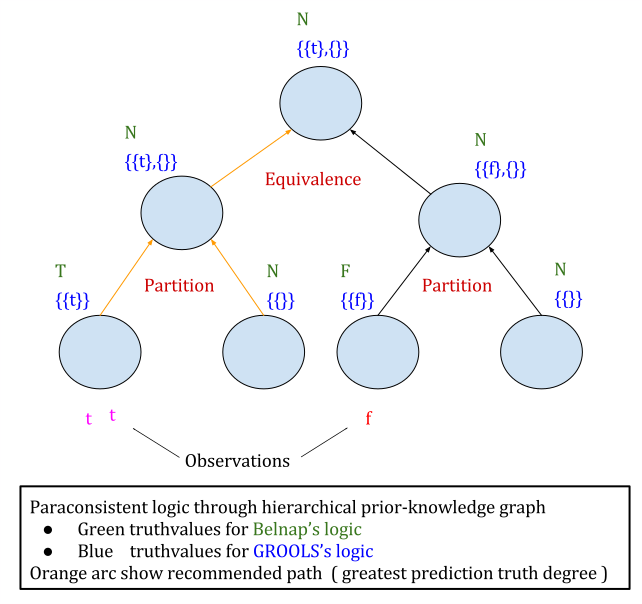
\includegraphics[width=\textwidth]{img/GROOLS_vs_belnap_1.pdf}
		\caption{Avec la logique de Belnap il n'est pas possible de suggérer le chemin le plus vraisemblable lorsqu'il y a des valeurs incertaines.}
		\label{fig:grools_belnap_1}
	\end{subfigure}
	\hfill
	\begin{subfigure}[t]{.48\textwidth}
		\centering
		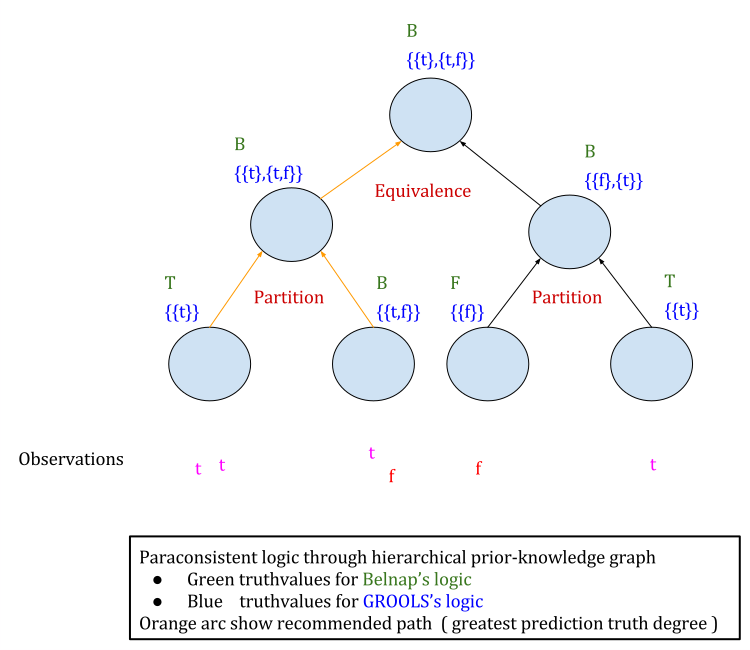
\includegraphics[width=\textwidth]{img/GROOLS_vs_belnap_2.pdf}
		\caption{Avec la logique de Belnap il n'est pas possible de distinguer le chemin avec le plus grand degré de véracité. }
		\label{fig:grools_belnap_2}
	\end{subfigure}
	\label{fig:grools_belnap}
\end{shadedfigure}

J'ai réalisé que la notion de valeur contradictoire décrite par Belnap ("Both") était en fait un ensemble de valeur de vérité vrai et fausse. Et par conséquent essayer de représenter un ensemble de plusieurs valeurs dans une seule valeur vérité "Both" était au mieux une approximation .

J'ai poursuivis mon idée sur les ensembles de valeur vérité et constaté que dans mon cas j'avais des ensembles d'observations. En effet, les sources d'observations peuvent être multiples et pour autant elles peuvent désigner le même concept. D'autre part, en laboratoire on peut être amené à répéter une même expérience. Il y a également le cas de figure avec des équipes différentes qui ont réalisé la même expérience. Et donc ces multiples observations bien que relié a une même théorie, elles peuvent avoir des résultats expérimentaux différents. Par conséquent les ensembles de valeur de vérité possibles en lien avec les ensembles d'observations sont : $\{t\} \{f\} \{t,f\} \{\emptyset\}$, respectivement ensemble : vrai, faux, vrai-et-faux, ni-vrai-ni-faux. 

Quant aux connaissances \textit{a priori}, elles sont observables par de multiple ensemble d'observations dû à la notion de composition de concepts. Pour illustrer, lorsqu'une connaissance \texttt{A} et composé d'une connaissance \texttt{B} et d'une autre \texttt{C}. Les observations relatives à la  connaissance \texttt{A}, c'est l'union des ensembles d'observations de \texttt{B} et \texttt{C} donc c'est un ensemble des parties d'un ensemble\footnote{En anglais on utilise le terme de "powerset"} d'observation. autrement dit, la prédiction de \texttt{A} est l'ensemble des sous-ensembles de prédits dans \texttt{B} et \texttt{C}. La combinaison des quatre ensembles d'observation ($\mathbb{P}(2)$) donne seize ensembles ($\mathbb{P}(4)$) par lesquels la predictabilité et l'expectabilité d'un concept peut être exprimé. Ces seize combinaisons permettent de mieux représenter la population des observations lié à un concept et ainsi faire des choix plus précis. Peu de temps après avoir décrit les seize ensembles possibles, j'ai remarqué qu'un travail de recherche similaire réalisé par \citeauthor{shramko2005some}. Ils décrivent ces mêmes ensembles, nommé les valeurs de vérités généralisés. Ces valeurs ont été présentées dans la partie \nameref{par:logic_multivalued}  à travers la \cref{fig:sixteen_truth_values}.

\needspace{5\baselineskip}
\begin{tasks}[counter-format = {tsk[1].},label-offset = {0.8em},label-format = {\bfseries}](4)
	\task $\{\emptyset\}$
	\task $\{\{\emptyset\}\}$
	\task $\{\{t\}\}$
	\task $\{\{f\}\}$
	\task $\{\{t,f\}\}$
	\task $\{\{t\},\{t,f\}\}$
	\task $\{\{\emptyset\},\{t\}\}$
	\task $\{\{\emptyset\},\{f\}\}$
	\task $\{\{t\},\{f\}\}$
	\task $\{\{f\},\{t,f\}\}$
	\task $\{\{\emptyset\},\{t\},\{t,f\}\}$
	\task $\{\{t\},\{f\},\{t,f\}\}$
	\task $\{\{\emptyset\},\{t\},\{f\}\}$
	\task $\{\{\emptyset\},\{t,f\}\}$
	\task $\{\{\emptyset\},\{f\},\{t,f\}\}$
	\task $\{\{\emptyset\},\{t\},\{f\},\{t,f\}\}$
\end{tasks}

Dans l'objectif de dissocier les observations qui émettent une prédictions de celles qui informe une expectation, chaque théorie possède deux espaces distincts (l'espace des prédictions et l'espace des expectations). Ces espaces sont représentés par des ensembles de valeurs de vérités $\mathbb{P}(4)$ . Les prédictions sont inférées vers les connaissances généralistes, c'est-a-dire des unités fonctionnelles vers les voies métaboliques et inversement pour les expectations. Lorsqu'au moins deux chemins équivalent se présentent, L'inférence des prédictions et des expectations peut être conditionné selon le degré de véracité ou de fausseté. Par exemple si une voie métaboliques est déclaré comme non attendues, alors tous les chemins menant à cette voie sont tous non attendues. Le degré de croyance peut être utilisé pour inférer les prédictions vers une voie métabolique requise lorsque qu'il existe plusieurs chemins équivalent (variant), par exemple si un chemin \texttt{A} est représenté par l'ensemble $\{\{t,f\}\}$ et un chemin  \texttt{B} représenté par l'ensemble $\{\{f\}\}$ alors le chemin \texttt{A} est suggéré  car intuitivement il possède un degré de croyance plus grand.

L'avantage des ensembles c'est la possibilité de calculer un degré de croyance, que l'on appelle également degré de véracité. Pour ce faire le calcul ce fait en quatre étapes et débute par ce qu'elles représentes, c'est-à-dire les valeurs de vérité vrai et fausse. Le postulat de départ pose que la valeur vrai "\texttt{t}" sur l'échelle la de véracité vaut 1 et 0 pour la valeur faux "\texttt{f}".

\needspace{25\baselineskip}
\begin{enumerate}
    \item Constitution des ensembles $\mathbb{P}(2)$ (i.e $\{\emptyset\},\{t\},\{f\},\{t,f\}$)
    \item Calcul du degré de vérité pour les ensembles  $\mathbb{P}(2)$.
    \begin{equation*}
    \frac{1}{n} \sum_{i=1}x_{i}
    \begin{cases}
    \{\emptyset\} \to \frac{0}{1} = 0 \\
    \{t\} \to \frac{1}{1} = 1 \\
    \{f\} \to \frac{0}{1} = 0 \\
    \{t,f\} \to \frac{1+0}{2} = 0.5
    \end{cases}
    \end{equation*}
    \item Constitution des ensembles $\mathbb{P}(4)$ (i.e les 16 ensembles).
    \item Calcul du degré de vérité pour les ensembles  $\mathbb{P}(4)$ . Chaque sous-ensemble est représenté par son degré de vérité (ex: $\{\{t\}.verit\acute{e},\{f\}.verit\acute{e}\}$). Quelques exemples:
    \begin{equation*}
    \frac{1}{n} \sum_{i=1}x_{i}.verit\acute{e}
    \begin{cases}
    \{\{t\}\}                               &\to \frac{1}{1} = 1 \\
    \{\{t,f\}\}                             &\to \frac{1}{2} = 0.5 \\
    \{\{t\},\{t,f\}\}                       &\to \frac{1+0.5}{2} = 0.75 \\
    \{\{\emptyset\},\{t\}\}                 &\to \frac{0+1}{2} = 0.5 \\
    \{\{t\},\{f\}\}                         &\to \frac{1+0}{2} = 0.5 \\
    \{\{\emptyset\},\{t\},\{f\},\{t,f\}\}   &\to \frac{0+1+0+0.5}{4} = 0.125
    \end{cases}
    \end{equation*}
\end{enumerate}

Cette méthode de calcul permet de calculer également le degré de fausseté (i.e non-croyance). Pour des ensembles  $\mathbb{P}(2)$ et au delà on peut calculer, (i) le degré de contradiction (1 pour le sous-ensemble $\{t,f\}$ et 0 pour les autres), (ii) le degré d'incertitude(1 pour le sous-ensemble $\{\emptyset\}$ et 0 pour les autres).

\begin{shadedfigure}[H]
    \centering
    \includegraphics[width=\textwidth]{img/set_3d.png}
    \caption{Représentation des ensembles  $\mathbb{P}(4)$ selon 3 axes, (i) vérité, (ii) fausseté, (iii) information (i.e le nombre de sous-ensemble).}
    \label{fig:set3d}
\end{shadedfigure}

\section{La méthode}\label{sec:methode}

Mes recherches m'ont conduit à développer une méthode pour représenter et raisonner sur des ensembles de valeurs de vérité. Lesquels sont utilisés pour décrire les prédictions et les expectations des différentes théories.

Dans l'article ci-dessous je décris comment inférer les prédictions et les expectation à travers un graphe de connaissances reliés les une aux autres pour exprimer soit la composition soit l'équivalence.




\section{Discussion}
\subsection{Difficulté rencontrée}
La description du raisonnement dans un système à base de règles a engendré quelques difficultés. La première est la non maitrise du moment de l'évaluation d'un groupe de fait par une règle. Il faut savoir que seul le moteur de règle décide quelle règle doit être activée à tel moment. Les conflits de priorités entre les règles est géré par \texttt{DROOLS} en interne( dit système de résolution de conflit). Il arrive par exemple que deux règles pourraient être activé à un même moment car la contrainte primaire est identique. Pour illustrer un tel cas, considéré les deux règles suivantes:

\needspace{25\baselineskip}
\begin{lstlisting}[style=drl-style,caption=conflit]
rule "Direct prediction"
when
	$k : PriorKnowledge(  )
	$p : Observation( type = Type.PREDICTION,  value != $k.prediction )
then
	modify($k){
		prediction = $p.value
	}
end

rule "Infer prediction from children PriorKnowledge"
when
	$k    : PriorKnowledge(  )
	$child: PriorKnowledge( $k memberOf parents, prediction not in $k.prediction )
then
	modify($k){
		prediction += $child.prediction
	}

end
\end{lstlisting}

Les deux règles ont la même contrainte primaire, c'est-à-dire de trouver l'existence d'une connaissance \textit{a priori}. Si une connaissance \textit{a priori} corresponds aux deux contraintes alors le moteur de règle décidera quelle règle doit être activée en premier. Ceci peut changer complétement le résultat, si  initialement elle possède une prédiction $\{\{t,f\}\}$, le concept enfant  $\{\{f\}\}$ et la prédiction directe $\{\{t\}\}$ alors lorsque la règle 1 puis 2 est activée la connaissance \$k a une prédiction  $\{\{t\},\{t,f\}\}$ et si c'est la règle 2 puis 1 on obtient:  $\{\{t\}\}$.

Il existe le système de \texttt{salience} qui attribue un poids a une règle et ainsi priorise les règles les une par rapport aux autres. La \texttt{salience} permet d'indiquer quelle règle doit être activé en privilégier. Mais avoir recours à la \texttt{salience}  est souvent le signe d'un raisonnement mal formulé. 

De surcroît, dans un système réactif, la modification de la connaissance \textit{a priori} induit par les deux règles provoque une boucle de raisonnement car elles vont perpétuellement s'activer. Pour éviter de tel cas de figure il faut rendre les règles plus précises, ce qui se traduit bien souvent par plus de règles pour correspondre à la diversité des possibilités. En conséquence  il y a un risque plus important de collision de règle, car il faut garantir a chaque ajout nouvel de règle qu'il n'existe de conflit au regard de toutes les autres règle et au regard de la diversité des faits possibles. Tout ceci rends la construction d'un raisonnement réactif très compliqué. Dans le cas précédemment décrit, la règle  pour l'inférence directe de la  prédiction peut être divisé en deux règles, la première pour inférer l'ensemble d'observation lorsque la connaissance \textit{a priori} ne possèdent aucune prédiction ($\{\{\emptyset\}\}$) et une seconde lorsque la connaissance \textit{a priori} possède une prédiction, les observations directes viennent s'ajouter à l'ensemble des prédictions.

Une des grandes difficultés lorsque l'on travaille avec ce type d'outil, c'est que nous obtenons un résultat final sans être en mesure d'identifier quelles règles ont été activé et pourquoi elles l'ont étaient. Le système \texttt{DROOLS} fournit un système de trace des évènements mais il est compliqué à analyser. Il n'indique pas pourquoi la règle est activé et encore moins pourquoi elle n'a pas était activé. Pour un petit jeu de données, les traces produises un volume important d'évènement, ce qui demande du temps pour les analyser et comprendre les choix du raisonneur. Autant dire que s'il existe un cas non souhaitais dues a une combinaison d'activation de plusieurs règles, c'est extrêmement laborieux d'analyser les traces.

En plus des difficultés pour cordonner les différentes règles, j'ai rencontré des erreurs critique dans le système \texttt{DROOLS} . Ces problèmes ont été rapporté aux développeurs quand j'était en mesure de fournir un exemple minimal, ce qui n'a pas était toujours le cas, car il est difficile de déterminer le contexte et l'ensemble minimal de règles nécessaire à reproduire le "bug". Ci-dessous je présente deux bugs que j'ai découvert avec la description d'un cas minimal  qui ont été rapporté à l'équipe de développement de \texttt{DROOLS}:
\begin{itemize}
	\item \url{https://issues.jboss.org/browse/DROOLS-809}
	\item \url{https://issues.jboss.org/browse/DROOLS-809}
\end{itemize}
 
En plus de devoir exprimer des contraintes sur les règles le système me contraignais sur la façon dont je pouvais les exprimer à cause de ces "bugs".

Malgré toutes ces difficultés, ce travail a aboutis à une version fonctionnelle \url{https://github.com/Grools/grools-drools-checker} . Cependant le raisonneur \texttt{DROOLS} a montré ces limites pour raisonner sur des données hiérarchiques. Les règles et les faits ne sont pas utilisés dans un ordre optimum vis-à-vis du graphe de connaissances, engendrant de nombreuses ré-activations de règles et donc un temps de calcul accrue. Mais également l'évaluation de collection de faits (essentiel pour le raisonnement), est très couteux pour le raisonneur \texttt{DROOLS}. Ces opérations bien que  possibles par le langage logique de \texttt{DROOLS}, notamment par les expressions \lstinline[style=drl-style]$Set() from collect(...)$, \lstinline[style=drl-style]$forall(...)$, \lstinline[style=drl-style]$Number() from accumulate(...)$ empêche le raisonneur d'activé les règles de façon efficace car la collection d'objet est crée qu'aprés l'activation de la règle. De plus à chaque réactivation de la même règle la même collection d'objet doit être recrée, ce qui est inefficace.  Le raisonnement prends entre 2 et 9 heures de calcul selon la quantité de fait et la représentation des connaissances utilisées (Genome-Properties, UniPathway). Il était donc nécessaire d'ajouter en plus du raisonnement de l'intelligence sur comment et quand activer les règles vis-à-vis d'un graphe de connaissances. J'avais commencé ce travail, mais là encore j'ai était confronté à des comportements indésirables de la part du raisonneur. J'ai établi au cours de ces trois années de bonne relation avec l'équipe de \texttt{DROOLS} . À la suite de la présentation  des nouveaux problèmes rencontré, ils m'ont proposé de travailler conjointement pour apporter les corrections dans la version suivante. Malheureusement le temps qui m'était impartit ne me permettait pas d'investiguer dans le moteur d'inférence, de trouver une solution, de la faire valider et d'attendre la nouvelle version.

C'est la raison pour laquelle j'ai ré-écrit un système réactif en pure Java. Afin de rester dans le contexte d'une programmation déclarative les règles ont été écrite en utilisant le paradigme de la programmation fonctionnelle\footnote{Qui perçoit les applications comme un ensemble de fonctions mathématiques, source: wikipedia}\footnote{\url{https://fr.wikipedia.org/wiki/Programmation_déclarative}}. Ce projet open source est appelé \texttt{grools-reasoner} (\url{https://github.com/Grools/grools-reasoner}). Cette bibliothèque a été utilisée pour l'exploration des voies métabolique de 14 génomes bactérien dans l'article présenté dans la \namecref{sec:methode} \cref{sec:methode}. L'outil s'est montré capable de raisonner sur tout un génome en moins d'une minute.

La bibliothèque est modulaire, elle peut être utilisée selon les différents besoins, comme:\nolisttopbreak
\begin{itemize}
	\item \texttt{grools-application} pour l'exploration du métabolisme à travers les modèles GenProperties,Unipathway  (\url{https://github.com/Grools/grools-application}).
	\item \texttt{grools-interpreter} pour charger un ancien raisonnement et effectué des requêtes pour l'analyses des faits (\url{https://github.com/Grools/grools-interpreter}).
	\item et d'autres à venir \ldots
\end{itemize}

\subsection{Logique para-cohérente}
Lorsqu'il est nécessaire de raisonner dans un monde avec des incertitudes et des incohérences, la logique à quatre valeurs de \textit{Belnap} semble suffisante. En effet, les valeurs de vérités $\{t\} \{f\} \{t,f\} \{\emptyset\}$ couvrent la notion de vraie, faux, contradictoire et incertain, cependant lorsque l'on regarde de plus près la table vérité  (voir la section \nameref{par:logic_multivalued}  \cref{tab:belnap_truth_table}) certaines combinaisons peuvent se montrer contre-intuitives, par exemple: $ BOTH \lor  NONE = TRUE$ et $ BOTH \land NONE = FALSE$. Le premier cas  peut se représenter de la sorte: 
\begin{itemize}
    \item Un variant \texttt{A} possède des prédictions contradictoire (BOTH).
    \item Un variant \texttt{B} a une absence de prédiction (NONE).
\end{itemize}
Lors du choix entre le variant \texttt{A} ou \texttt{B} d'après la table de vérité de \textit{Belnap} la voie métabolique serait prédite (TRUE). Ce résultat non-intuitif est dû a une impossibilité d'exprimer plus de quatre états. Mais également le fait de considérer des ensembles de valeur de vérité comme des valeur de vérité à part entière. Cette logique essaye de représenter l'ensemble $\{t,f\}$ qui comporte deux valeurs en une seule, ce qui inexorablement amènent à des approximations. Cette logique ne peut donc pas être utilisée avec un graphe de connaissance sans amené des  imprécisions comme montré avec la \cref{fig:grools_belnap_1} et la  \cref{fig:grools_belnap_2}. 

A mon avis, ces ensembles de valeurs de vérités ne sont pas des valeurs de vérités. Par conséquent il ne faut pas essayer d'étendre la logique classique à d'autres valeurs de vérités. Ce point de vue rejoint celui émis par \citeauthor{dubois2008ignorance} dans \citetitle{dubois2008ignorance}\cite{dubois2008ignorance}. La logique multi-valuée de Belnap a introduit une confusion entre valeur de vérité et l'état d'information.



\subbibliography
\end{refsegment}